\section{Optimal Offline Algorithm for Model $1$}\label{sec:offline-optimal-algorithm}

The problem can be modelled as an instance of the minimum cost flow network. We define the minimum cost flow problem here for completeness. 

\paragraph{The minimum cost flow problem:} The input is a flow network $G=(V,E)$ as a directed graph with node set $V$, edge set $E$, capacities $c_e>0$ and cost $u_e\in \mathbb{R}$ on each edge $e\in E$, and a source $s$ and sink $t$. A flow $f:E\rightarrow \mathbb{R}$ is a valid flow in $G$ if $f(e)\leq c(e)$, and the incoming flow at any node except $s$ and $t$ equals the outgoing flow. The cost of a flow $f(e)$ along an edge $e$ is
$u_e\cdot f(e)$. A minimum cost flow in the network is the one that minimizes the sum of costs of the flow along all edges.

There are polynomial-time algorithms known for the minimum cost flow problem. Also, it is known that if all the capacities are integers, then the optimum flow is an integer. We refer the reader to \cite{Ahuja93} for the details of minimum cost flow. 
\paragraph{Reduction: }
The construction of the flow network is shown in Figure~\ref{fig:flow-nw}. The flow network consists of a source $s$, a sink $t$, nodes for each day $d_j$, each agent $a_k$ and nodes $c_{ij}$ for each $(c_i,d_j)\in C\times D$. Each edge $(s,d_j)$ has capacity $s_j$ denoting the daily supply for day $d_j$, each edge $(d_j,c_{ij})$ has capacity equal to $q_{ij}$, and all other edges have capacity $1$. All the edges are directed. Additionally, each $(c_{ij},a_k)$ edge has cost $-u_k\cdot\delta_k^j$ whereas other edges have cost $0$.

\begin{proof}(of Theorem~\ref{thm:off-opt})
We show that a minimum cost flow $f$ in the flow network corresponds to a maximum utility matching in the given instance. The integrality of minimum cost flow implies that each edge incident on $t$ can have a flow of either $0$ or $1$. For each $k$, if $f(a_k,t)=1$, then 
there is exactly one $c_{ij}$ such that $f(c_{ij},a_k)=1$. Set $M(a_k)=(c_i,d_j)$ in the
corresponding matching $M$. Similarly, for any matching $M$, A corresponding flow  can be shown as follows. If $M(a_k)=(c_i,d_j)$ then set $f(a_k,t)=f(c_{ij},a_k)=1$, and set $f(s,d_j)$ equal to the number of agents vaccinated on day $d_j$, and $f(d_j,c_{ij})$ equal to the number of agents vaccinated on day $d_j$ through category $c_i$. It is clear that this is a valid flow in the network, and the negation of the cost of the flow is the same as the utility of the corresponding matching.
\end{proof}

\begin{figure}
  \centering
  \scalebox{1}{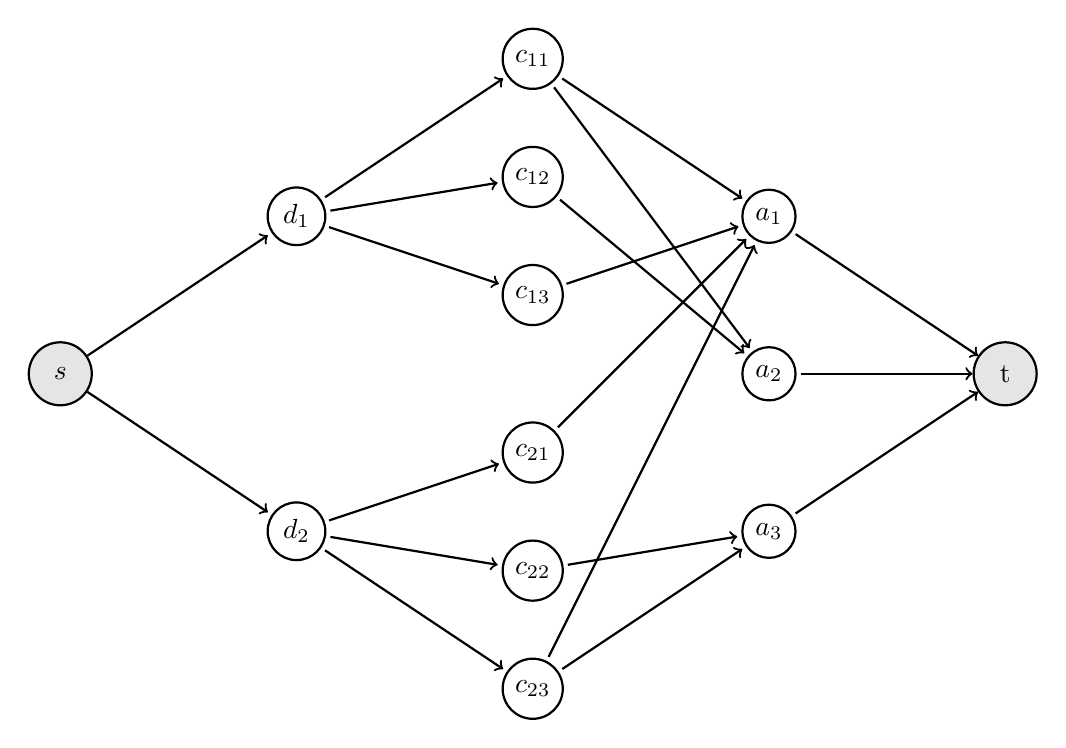
\begin{tikzpicture}[myn/.style={circle,thick,draw,inner sep=.1cm,outer sep=2pt},scale = 1,
      terminal/.style={circle, draw=black, fill=black!10, thick, minimum size=8mm},
      ]

      \node[terminal] (s) at (0,0) {$s$};
      \node[myn] (d1) at (3,2) {$d_1$};
      \node[myn] (d2) at (3,-2) {$d_2$};
      \node[myn] (c11) at (6,4) {$c_{11}$};
      \node[myn] (c12) at (6,2.5) {$c_{12}$};
      \node[myn] (c13) at (6,1) {$c_{13}$};
      \node[myn] (c21) at (6,-1) {$c_{21}$};
      \node[myn] (c22) at (6,-2.5) {$c_{22}$};
      \node[myn] (c23) at (6,-4) {$c_{23}$};
      \node[myn] (a1) at (9,2) {$a_1$};
      \node[myn] (a2) at (9,0) {$a_2$};
      \node[myn] (a3) at (9,-2) {$a_3$};
      \node[terminal] (t) at (12,0) {t};
      \draw[thick, ->] (s)--(d1);
      \draw[thick, ->] (s)--(d2);
      \draw[thick, ->] (d1)--(c11);
      \draw[thick, ->] (d1)--(c12);
      \draw[thick, ->] (d1)--(c13);
      \draw[thick, ->] (d2)--(c21);
      \draw[thick, ->] (d2)--(c22);
      \draw[thick, ->] (d2)--(c23);
      \draw[thick, ->] (c11)--(a1);
      \draw[thick, ->] (c13)--(a1);
      \draw[thick, ->] (c21)--(a1);
      \draw[thick, ->] (c23)--(a1);
      \draw[thick, ->] (c11)--(a2);
      \draw[thick, ->] (c12)--(a2);
      \draw[thick, ->] (c22)--(a3);
      \draw[thick, ->] (c23)--(a3);
      \draw[thick, ->] (a1)--(t);
      \draw[thick, ->] (a2)--(t);
      \draw[thick, ->] (a3)--(t);
    \end{tikzpicture}}
  \caption{Flow network for finding a maximum utility matching in Model 1}
\end{figure}\label{fig:flow-nw}
% note for self: a_1 is available on both days and belong to the first and third category. a_2 is available on day 1 and belongs to category 1 and 2. a3 is available only in category 2 and 3 and available on day 2 only
